%\documentclass[handout]{beamer}
\documentclass[10pt]{beamer}
%for(int i=0; i<n; i++){\documentclass[10pt,handout]{beamer}
\usepackage[spanish]{babel}
% % \usepackage[backend=biber, style=authoryear-icomp]{biblatex}
\resetcounteronoverlays{exx}
\usepackage{mdframed}
\usepackage{tikz}
\usepackage{blindtext}
\usepackage{tipa}
% \usepackage{cgloss4e}
% \usepackage{gb4e}
% \usepackage{qtree}
\usepackage{cancel}
\usepackage{wrapfig}
\usepackage{soul}
\usepackage{enumerate}
\usepackage{longtable}
\graphicspath{ {./figures/} } % declaramos donde estan las imagenes
\usepackage[labelformat=simple]{subcaption} % para varias imagenes juntas
\renewcommand\thesubfigure{(\alph{subfigure})}
\usepackage[utf8]{inputenc}
\usepackage{amsmath}
\usepackage{amsfonts} % simbolos como el I de matriz identidad
\usepackage{bm}
\usepackage{graphicx} % paquete para ver imagenes
\usepackage{setspace}
\usepackage[T1]{fontenc}
\usepackage{parskip}
\usepackage{color}
\usepackage{framed}

\usetheme{Copenhagen}
\definecolor{frenchblue}{rgb}{0.0, 0.45, 0.73} % ESTE!!!!
\setbeamercolor{block body}{bg=frenchblue!50}
\setbeamercolor*{structure}{fg=frenchblue,bg=blue}
\setbeamercolor{normal text}{fg=black}
\setbeamercolor{frametitle}{bg=black}
\setbeamertemplate{frametitle}[default][center]
\setlength{\parskip}{12pt}
\useoutertheme{infolines} % me comia mucho espacio de la otra fgorma
\makeatother
\setbeamertemplate{footline}
{
  \leavevmode%
  \hbox{%
  \begin{beamercolorbox}[wd=.3\paperwidth,ht=2.25ex,dp=1ex,center]{author in head/foot}%
    \usebeamerfont{author in head/foot}\insertshortauthor
  \end{beamercolorbox}%
  \begin{beamercolorbox}[wd=.6\paperwidth,ht=2.25ex,dp=1ex,center]{title in head/foot}%
    \usebeamerfont{title in head/foot}\insertshorttitle
  \end{beamercolorbox}%
  \begin{beamercolorbox}[wd=.1\paperwidth,ht=2.25ex,dp=1ex,center]{date in head/foot}%
    \insertframenumber{} / \inserttotalframenumber\hspace*{1ex}
  \end{beamercolorbox}}%
  \vskip0pt%
}
\makeatletter
\setbeamertemplate{navigation symbols}{}
%\setbeameroption{show notes}
\setbeameroption{hide notes}
\renewcommand{\CancelColor}{\color{red}}

\usepackage{hyperref}

\title[RISC II]{Presentación RISC II}
\author[Matias Mazzanti]{Matias Mazzanti}


\institute{DC-UBA}
\date{05 de Septiembre de 2022}

\titlegraphic{
\includegraphics[,height=2cm,keepaspectratio]{../logo.pdf}     }
%\logo{
\includegraphics[height=2.5cm]{logo.PDF}}

\begin{document}

\begin{frame}

\maketitle

\end{frame}

% cuál es tu background que estuviste haciendo y qué querés hacer
% Con quién vas a trabajar en los planes
% un poquito de cuál es la idea del doctorado aunque todavía este verde

\section{Presentaci\'on}
\begin{frame}
\frametitle{Introducción}

\begin{itemize}
  \item Licenciado en Ciencias de la Física.
  \item Alumno doctoral de Esteban Mocskos: Laboratorio Interdisciplinario de Computación de Alto Rendimiento. UBA.
  \item Tema doctoral: Soporte en Hardware para FHE (Fully Homomorphic Encryption).
\end{itemize}

\end{frame}



\begin{frame}
\frametitle{Introducción}
\begin{figure}[h!]
    \centering
    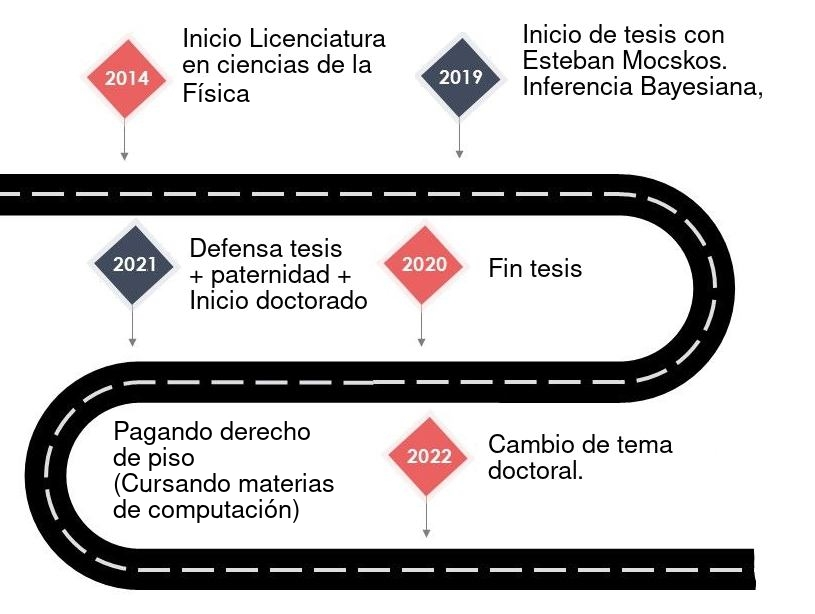
\includegraphics[scale=0.3]{road.jpg}
\end{figure}
\end{frame}


\begin{frame}
\frametitle{Orígenes y tesis}

 Durante la Lic Física me acerqué a la computación (materias optativas).
\begin{columns}
    \column{0.5\textwidth}
\vspace{0.5cm}
\pause

Tesis dentro del departamento de computación de la UBA.
\vspace{0.5cm}

Estimaciones Bayesianas de la habilidad en jugadores del juego de mesa de Go.

\vspace{0.5cm}
\pause
Se propuso una mejora en el sistema de rankeo para plataformas online.
    \column{0.5\textwidth}
\begin{figure}[h!]
    \centering
    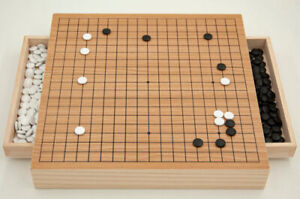
\includegraphics[scale=2.]{go.jpg}
\end{figure}
\end{columns}
\end{frame}

\begin{frame}
\frametitle{Doctorado}
Propuesta original: Continuar el tema de la tesis utilizando el modelo de estimación y buscar su paralelización mediante GPU.

\pause
La paralelización para el modelo no se justificaba $\rightarrow$ utilizar el modelo para responder otras preguntas.

\pause
Modelar y estudiar el aprendizaje humano.

\pause
El camino que tomó el doctorado  no me convenció $\to$ cambio de planes.



\end{frame}

\begin{frame}
\frametitle{Cambio Doctorado}
        \vspace{0.3cm}

\begin{columns}
    \column{0.5\textwidth}
        Director: Esteban Mocskos UBA
        \vspace{0.3cm}

        Codirector: Augusto Vega IBM

        \vspace{0.3cm}
        Fully Homomorphic Encryption (FHE).

\pause
        \vspace{0.3cm}
        Operar \textbf{directamente} con datos encriptados (sin necesidad de desencriptar).


    \column{0.5\textwidth}
\begin{figure}[h!]
    \centering
    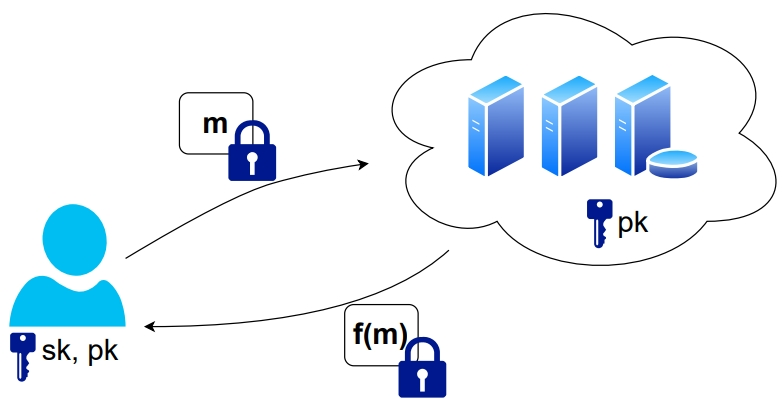
\includegraphics[scale=0.19]{fhe.jpg}
\end{figure}
\end{columns}


\pause
Ej: Lograr procesar remotamente con machine learning sin revelar los datos.
 \vspace{-0.25cm}

Potencialmente con mucha utilidad para uso de cloud computing.
 \vspace{-0.15cm}

\pause
Actualidad: ordenes de magnitud lento para uso real.
 \vspace{-0.15cm}

\pause
\begin{mdframed}[backgroundcolor=frenchblue!20]\centering
  Acelerar mediante hardware.
\end{mdframed}

\end{frame}


%Complejidad de FHE,

%Por que se requiere aceleracion por hardware

%Costos computacionales

%Limites




\begin{frame}
\frametitle{FHE}
\begin{columns}
    \column{0.6\textwidth}
    Requierimientos y problemas FHE:
\pause
\begin{itemize}
  \item[\textcolor{frenchblue}{\textbullet}] Homomorfismo en la suma y multiplicación.
    \begin{itemize}
\pause
      \item[\textcolor{red}{\textbullet}]  No todo esquema es homomorfico en ambas operaciones.
    \end{itemize}
\pause
  \item[\textcolor{frenchblue}{\textbullet}] Ilimitada cantidad de operaciones.
    \begin{itemize}
\pause
      \item[\textcolor{red}{\textbullet}]  La mayoría de esquemas utilizan \texttt{Learning With Errors} (LWE). Aumentando su error por cada operación (principalmente en multiplicaciones).
    \end{itemize}
\pause
  \item[\textcolor{frenchblue}{\textbullet}] Tiempos razonables
    \begin{itemize}
\pause
      \item[\textcolor{red}{\textbullet}]  Los esquemas actuales tienen un costo muy grande por cada operación: orden del segundo.
    \end{itemize}
\end{itemize}
    \column{0.4\textwidth}
\pause
        \begin{figure}[h!]
            \centering
            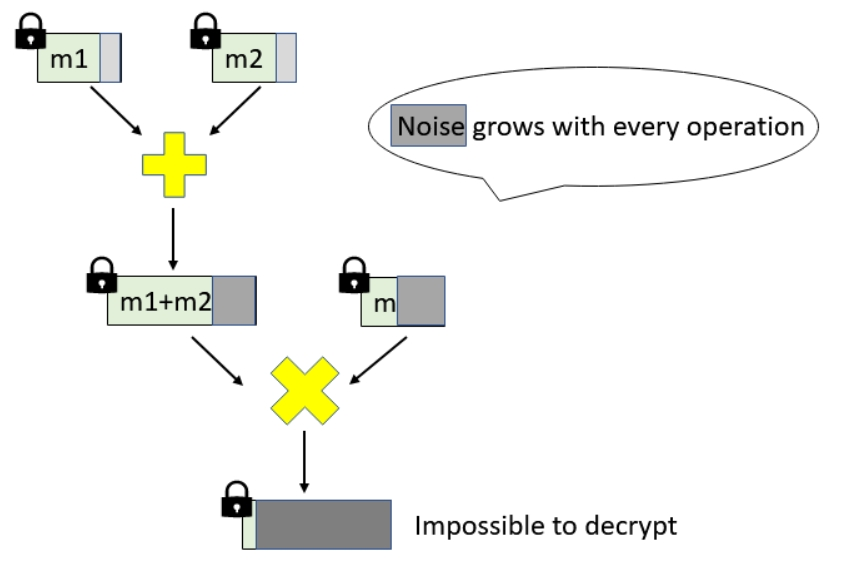
\includegraphics[scale=0.2]{multNoise.jpg}
        \end{figure}

\end{columns}
\pause
        Cada operación homomórfica es $10^3 \sim 10^6$ veces más lento que sin  encriptar.


\end{frame}


\begin{frame}
\frametitle{Bootstrapping}
Gentry (2009) $\to$ primer  esquema FHE mediante \texttt{Bootstrapping}: reducir el error luego de una operación.

\pause
Actualiza el cifrado produciendo un nuevo cifrado del mismo mensaje pero con menor ruido.

\pause
Descifrar homomorficamente: se vuelve a encriptar utilizando como clave la clave secreta encriptada.

\pause
Operación muy costosa: principal cuellos de botella de FHE.



\pause
\begin{mdframed}[backgroundcolor=frenchblue!20]
  Bootstrapping, más otros métodos para reducir ruido, representan el 95\% del esfuerzo computacional y movimientos de data.
\end{mdframed}
\end{frame}

  \begin{frame}
\frametitle{Esquema simplificado}
En general: Se trabaja con mensajes vectoriales $\to$ SIMD.
    \vspace{-0.3cm}

\pause
  Pasos (simplifacacion del esquema CKKS):
    \vspace{-0.3cm}
\begin{itemize}
  \item Anillo polinomial de orden alto ($2^{10} \sim 2^{18}$).
\pause
    \vspace{-0.3cm}
  \item Se codifica a textoplano m(X) a un polinomio del anillo.
\pause
    \vspace{-0.3cm}
  \item Encriptar: ct = (b(X), a(X)) = (a(X)*s(X) + m(X) + e(X), a(X)). A polinomio aleatorio, s clave secreta, e error gausiano polinomial.
\pause
    \vspace{-0.3cm}
  \item Desencriptar ct: m$'$(X)= ct*(1,-s(X)) = m(X)+e(X) (buena aprox si e es chico).
\pause
    \vspace{-0.3cm}
  \item Suma ct$_1$ + ct$_2$: (b$_1$(X) + b$_2$(X), a$_1$(X) + a$_2$(X)).
\pause
    \vspace{-0.3cm}
  \item Mult ct$_1$*ct$_2$: (b$_1$*b$_2$, a$_1$*b$_2$+a$_2$*b$_1$, a$_1$*a$_2$). (Otro paso: cambio de clave, otra mult polinomial)
\pause
    \vspace{-0.3cm}
  \item Boostrapping: Cientos de Multiplicaciones homomorficas y shifteos circulares de bits.
\end{itemize}

\end{frame}


\begin{frame}
\frametitle{Conclusiones}
FHE es un tipo de encriptaciones muy costosa pero prometedora.

<<<<<<< HEAD
Otro problema es el consumo de memoria.
=======
>>>>>>> 1326c51 (Diapo CKKS)

\pause
Tiene un gran consumo de memoria:
\pause
Una mensaje homomorficamente encriptado puede ocupar $10^5$ más espacio y las claves encriptadas pueden llegar a los GBs.
Grandes movimientos de datos.

\pause
Alto costo computacional:
\pause
  Los esquemas FHE son iterativos con operaciones polinomiales de ordenes altos y coeficientes grandes ($\sim 1000$bits).

\pause
\begin{mdframed}[backgroundcolor=frenchblue!20]
  Arquitectura especializada: eficiencia en costo computacional y consumo de memoria.
\end{mdframed}

\end{frame}

\begin{frame}
\frametitle{}
  \begin{figure}[h!]
      \centering
      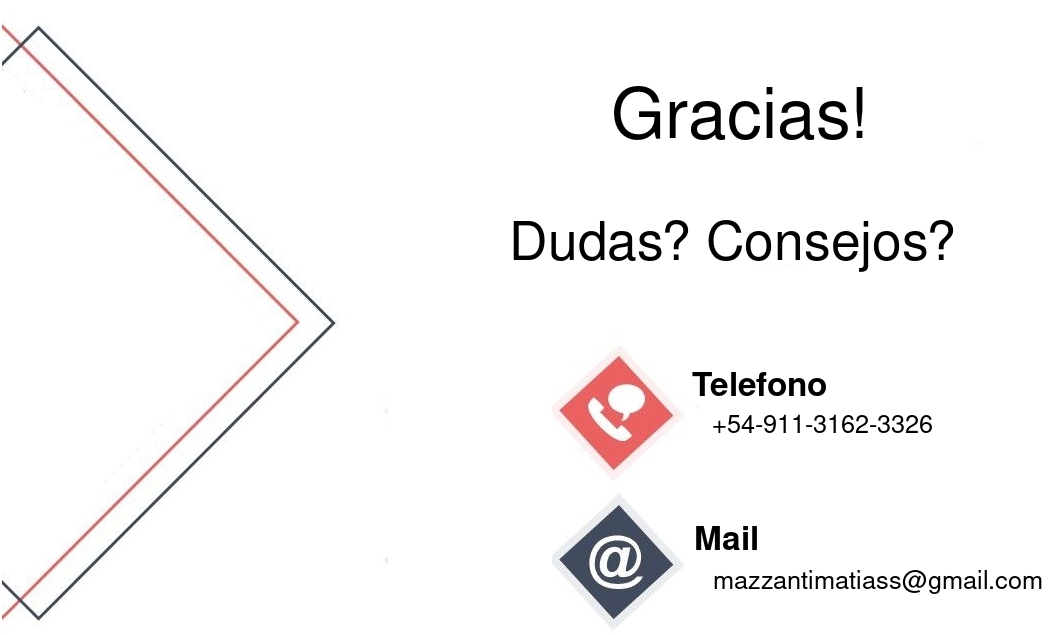
\includegraphics[scale=0.3]{agradecimientos.jpg}
  \end{figure}
\end{frame}



\end{document}
